%\documentclass[12pt]{scrbook}
%
%\usepackage{tikz}
%\usepackage{minted}
%%\usetikzlibrary{decorations.pathreplacing}
%%
%\usetikzlibrary{patterns}
%\usetikzlibrary{decorations.pathreplacing,arrows}
%\usetikzlibrary{arrows,decorations.pathmorphing,backgrounds,positioning,fit,petri}
%
%\usepackage{fullpage}
%\usepackage{subfigure}
%\begin{document}
%
%
%Lorem Ipsum is simply dummy text of the printing and typesetting industry. Lorem Ipsum has been the industry's standard dummy text ever since the 1500s, when an unknown printer took a galley of type and scrambled it to make a type specimen book. It has survived not only five centuries, but also the leap into electronic typesetting, remaining essentially unchanged. It was popularised in the 1960s with the release of Letraset sheets containing Lorem Ipsum passages, and more recently with desktop publishing software like Aldus PageMaker including versions of Lorem Ipsum.

\begin{figure}
\centering

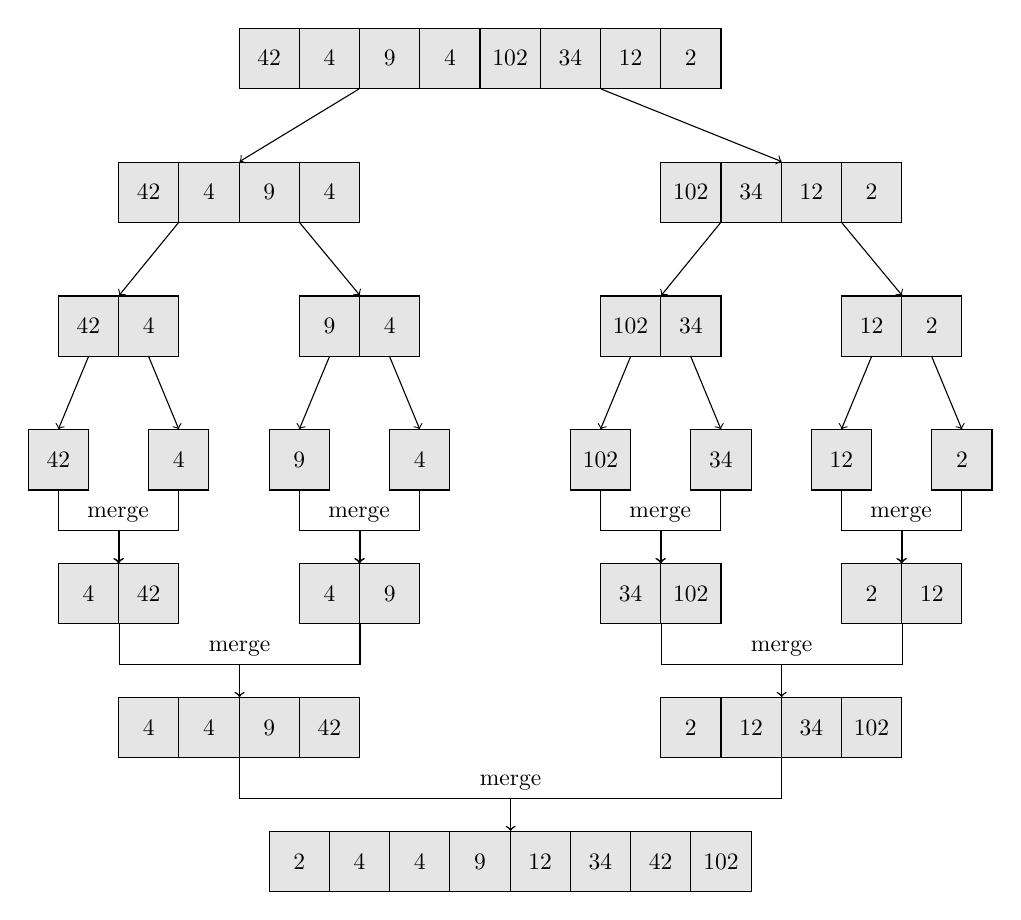
\begin{tikzpicture}[scale=.85,transform shape]

%\tikzset{>=stealth',shorten <=.2cm,>=stealth',shorten >=.2cm}
% size of each node
\def\sz{9mm}
% node style definition
\tikzstyle{block} = [
	draw, fill=black!10, rectangle,
	minimum height=\sz, minimum width=\sz ];
\tikzstyle{plain} = [draw=none,fill=none];

\node[block] (a0) at (0*\sz,0) { 42 };
\node[block] (a1) at (1*\sz,0) { 4 };
\node[block] (a2) at (2*\sz,0) { 9 };
\node[block] (a3) at (3*\sz,0) { 4 };
\node[block] (a4) at (4*\sz,0) { 102 };
\node[block] (a5) at (5*\sz,0) { 34 };
\node[block] (a6) at (6*\sz,0) { 12 };
\node[block] (a7) at (7*\sz,0) { 2 };

\node[block] (aa0) at (-2*\sz,-2) { 42 };
\node[block] (aa1) at (-1*\sz,-2) { 4 };
\node[block] (aa2) at (0*\sz,-2) { 9 };
\node[block] (aa3) at (1*\sz,-2) { 4 };

\node[block] (aa4) at (7*\sz,-2) { 102 };
\node[block] (aa5) at (8*\sz,-2) { 34 };
\node[block] (aa6) at (9*\sz,-2) { 12 };
\node[block] (aa7) at (10*\sz,-2) { 2 };

\node[block] (aaa0) at (-3*\sz,-4) { 42 };
\node[block] (aaa1) at (-2*\sz,-4) { 4 };

\node[block] (aaa2) at (1*\sz,-4) { 9 };
\node[block] (aaa3) at (2*\sz,-4) { 4 };

\node[block] (aaa4) at (6*\sz,-4) { 102 };
\node[block] (aaa5) at (7*\sz,-4) { 34 };

\node[block] (aaa6) at (10*\sz,-4) { 12 };
\node[block] (aaa7) at (11*\sz,-4) { 2 };

\node[block] (aaaa0) at (-3.5*\sz,-6) { 42 };
\node[block] (aaaa1) at (-1.5*\sz,-6) { 4 };
\node[block] (aaaa2) at (0.5*\sz,-6) { 9 };
\node[block] (aaaa3) at (2.5*\sz,-6) { 4 };

\node[block] (aaaa4) at (5.5*\sz,-6) { 102 };
\node[block] (aaaa5) at (7.5*\sz,-6) { 34 };
\node[block] (aaaa6) at (9.5*\sz,-6) { 12 };
\node[block] (aaaa7) at (11.5*\sz,-6) { 2 };

\draw[->] (a2.south west) -- (aa1.north east);
\draw[->] (a5.south east) -- (aa5.north east);

\draw[->] (aa1.south west) -- (aaa0.north east);
\draw[->] (aa2.south east) -- (aaa2.north east);
\draw[->] (aa5.south west) -- (aaa4.north east);
\draw[->] (aa6.south east) -- (aaa6.north east);

\draw[->] (aaa0.south) -- (aaaa0.north);
\draw[->] (aaa1.south) -- (aaaa1.north);
\draw[->] (aaa2.south) -- (aaaa2.north);
\draw[->] (aaa3.south) -- (aaaa3.north);
\draw[->] (aaa4.south) -- (aaaa4.north);
\draw[->] (aaa5.south) -- (aaaa5.north);
\draw[->] (aaa6.south) -- (aaaa6.north);
\draw[->] (aaa7.south) -- (aaaa7.north);

\node[block] (bbb0) at (-3*\sz,-8) { 4 };
\node[block] (bbb1) at (-2*\sz,-8) { 42 };

\node[block] (bbb2) at (1*\sz,-8) { 4 };
\node[block] (bbb3) at (2*\sz,-8) { 9 };

\node[block] (bbb4) at (6*\sz,-8) { 34 };
\node[block] (bbb5) at (7*\sz,-8) { 102 };

\node[block] (bbb6) at (10*\sz,-8) { 2 };
\node[block] (bbb7) at (11*\sz,-8) { 12 };

\node[block] (bb0) at (-2*\sz,-10) { 4 };
\node[block] (bb1) at (-1*\sz,-10) { 4 };
\node[block] (bb2) at (0*\sz,-10) { 9 };
\node[block] (bb3) at (1*\sz,-10) { 42 };

\node[block] (bb4) at (7*\sz,-10) { 2 };
\node[block] (bb5) at (8*\sz,-10) { 12 };
\node[block] (bb6) at (9*\sz,-10) { 34 };
\node[block] (bb7) at (10*\sz,-10) { 102 };

\node[block] (b0) at (0.5*\sz,-12) { 2 };
\node[block] (b1) at (1.5*\sz,-12) { 4 };
\node[block] (b2) at (2.5*\sz,-12) { 4 };
\node[block] (b3) at (3.5*\sz,-12) { 9 };
\node[block] (b4) at (4.5*\sz,-12) { 12 };
\node[block] (b5) at (5.5*\sz,-12) { 34 };
\node[block] (b6) at (6.5*\sz,-12) { 42 };
\node[block] (b7) at (7.5*\sz,-12) { 102 };

\draw[->] (aaaa0.south) -- ++(0,-0.6) -| (bbb0.north east);
\draw[->] (aaaa1.south) -- ++(0,-0.6) -| node[above] {merge} (bbb1.north west);
\draw[->] (aaaa2.south) -- ++(0,-0.6) -| (bbb2.north east);
\draw[->] (aaaa3.south) -- ++(0,-0.6) -| node[above] {merge} (bbb3.north west);
\draw[->] (aaaa4.south) -- ++(0,-0.6) -| (bbb4.north east);
\draw[->] (aaaa5.south) -- ++(0,-0.6) -| node[above] {merge} (bbb5.north west);
\draw[->] (aaaa6.south) -- ++(0,-0.6) -| (bbb6.north east);
\draw[->] (aaaa7.south) -- ++(0,-0.6) -| node[above] {merge} (bbb7.north west);

\draw[->] (bbb0.south east) -- ++(0,-0.6) -| (bb1.north east);
\draw[->] (bbb2.south east) -- ++(0,-0.6) -| node[above] {merge} (bb1.north east);
\draw[->] (bbb4.south east) -- ++(0,-0.6) -| (bb5.north east);
\draw[->] (bbb6.south east) -- ++(0,-0.6) -| node[above] {merge} (bb5.north east);

\draw[->] (bb1.south east) -- ++(0,-0.6) -| (b3.north east);
\draw[->] (bb5.south east) -- ++(0,-0.6) -| node[above] {merge} (b3.north east);

\end{tikzpicture}

\caption[Merge Sort Example]{Illustration of Merge Sort's recursion and
merge operations.}
\label{figure:mergeSortExample}
\end{figure}

\begin{figure}
\centering

\subfigure[Iteration One.  $L_1 = 4 > R_1 = 2$, so the element
in the right partition is copied into $A_1$.  Both $j, k$ are
incremented.]{

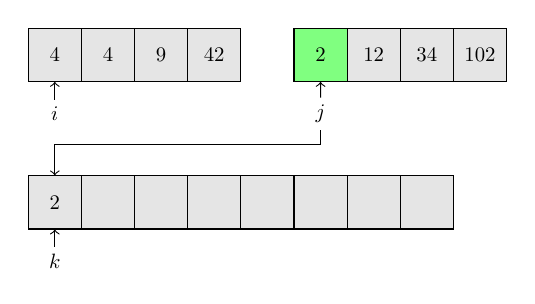
\begin{tikzpicture}[scale=.75,transform shape]

%\tikzset{>=stealth',shorten <=.2cm,>=stealth',shorten >=.2cm}
% size of each node
\def\sz{9mm}
% node style definition
\tikzstyle{block} = [
	draw, fill=black!10, rectangle,
	minimum height=\sz, minimum width=\sz ];
\tikzstyle{plain} = [draw=none,fill=none];

\node[block] (b0) at (0*\sz,0) { 4 };
\node[block] (b1) at (1*\sz,0) { 4 };
\node[block] (b2) at (2*\sz,0) { 9 };
\node[block] (b3) at (3*\sz,0) { 42 };

\node[block,fill=green!50] (b4) at (5*\sz,0) { 2 };
\node[block] (b5) at (6*\sz,0) { 12 };
\node[block] (b6) at (7*\sz,0) { 34 };
\node[block] (b7) at (8*\sz,0) { 102 };

\node[below of=b0] (i) {$i$};
\node[below of=b4] (j) {$j$};

\draw[->] (i) -- (b0);
\draw[->] (j) -- (b4);

\node[block] (a0) at (0*\sz,-2.5) { 2 };
\node[block] (a1) at (1*\sz,-2.5) {  };
\node[block] (a2) at (2*\sz,-2.5) {  };
\node[block] (a3) at (3*\sz,-2.5) {  };
\node[block] (a4) at (4*\sz,-2.5) {  };
\node[block] (a5) at (5*\sz,-2.5) {  };
\node[block] (a6) at (6*\sz,-2.5) {  };
\node[block] (a7) at (7*\sz,-2.5) {  };

\node[below of=a0] (k) {$k$};
\draw[->] (k) -- (a0);

\draw[->] (j.south) -- ++(0,-0.25) -| (a0.north);

\end{tikzpicture}
}~~~~~\subfigure[Iteration Two.  Now the element in the left
partition is lesser and is copied, incrementing $i, k$]{

\begin{tikzpicture}[scale=.75,transform shape]

%\tikzset{>=stealth',shorten <=.2cm,>=stealth',shorten >=.2cm}
% size of each node
\def\sz{9mm}
% node style definition
\tikzstyle{block} = [
	draw, fill=black!10, rectangle,
	minimum height=\sz, minimum width=\sz ];
\tikzstyle{plain} = [draw=none,fill=none];

\node[block,fill=green!50] (b0) at (0*\sz,0) { 4 };
\node[block] (b1) at (1*\sz,0) { 4 };
\node[block] (b2) at (2*\sz,0) { 9 };
\node[block] (b3) at (3*\sz,0) { 42 };

\node[block,pattern=north west lines, pattern color=blue] (b4) at (5*\sz,0) { 2 };
\node[block] (b5) at (6*\sz,0) { 12 };
\node[block] (b6) at (7*\sz,0) { 34 };
\node[block] (b7) at (8*\sz,0) { 102 };

\node[below of=b0] (i) {$i$};
\node[below of=b5] (j) {$j$};

\draw[->] (i) -- (b0);
\draw[->] (j) -- (b5);

\node[block] (a0) at (0*\sz,-2.5) { 2 };
\node[block] (a1) at (1*\sz,-2.5) { 4 };
\node[block] (a2) at (2*\sz,-2.5) {  };
\node[block] (a3) at (3*\sz,-2.5) {  };
\node[block] (a4) at (4*\sz,-2.5) {  };
\node[block] (a5) at (5*\sz,-2.5) {  };
\node[block] (a6) at (6*\sz,-2.5) {  };
\node[block] (a7) at (7*\sz,-2.5) {  };

\node[below of=a1] (k) {$k$};
\draw[->] (k) -- (a1);

\draw[->] (i.south) -- ++(0,-0.25) -| (a1.north);

\end{tikzpicture}
}

\subfigure[Iteration Three.  Again the element in the
left partition is less.]{

\begin{tikzpicture}[scale=.75,transform shape]

%\tikzset{>=stealth',shorten <=.2cm,>=stealth',shorten >=.2cm}
% size of each node
\def\sz{9mm}
% node style definition
\tikzstyle{block} = [
	draw, fill=black!10, rectangle,
	minimum height=\sz, minimum width=\sz ];
\tikzstyle{plain} = [draw=none,fill=none];

\node[block,pattern=north west lines, pattern color=blue] (b0) at (0*\sz,0) { 4 };
\node[block,fill=green!50] (b1) at (1*\sz,0) { 4 };
\node[block] (b2) at (2*\sz,0) { 9 };
\node[block] (b3) at (3*\sz,0) { 42 };

\node[block,pattern=north west lines, pattern color=blue] (b4) at (5*\sz,0) { 2 };
\node[block] (b5) at (6*\sz,0) { 12 };
\node[block] (b6) at (7*\sz,0) { 34 };
\node[block] (b7) at (8*\sz,0) { 102 };

\node[below of=b1] (i) {$i$};
\node[below of=b5] (j) {$j$};

\draw[->] (i) -- (b1);
\draw[->] (j) -- (b5);

\node[block] (a0) at (0*\sz,-2.5) { 2 };
\node[block] (a1) at (1*\sz,-2.5) { 4 };
\node[block] (a2) at (2*\sz,-2.5) { 4 };
\node[block] (a3) at (3*\sz,-2.5) {  };
\node[block] (a4) at (4*\sz,-2.5) {  };
\node[block] (a5) at (5*\sz,-2.5) {  };
\node[block] (a6) at (6*\sz,-2.5) {  };
\node[block] (a7) at (7*\sz,-2.5) {  };

\node[below of=a2] (k) {$k$};
\draw[->] (k) -- (a2);

\draw[->] (i.south) -- ++(0,-0.25) -| (a2.north);

\end{tikzpicture}
}~~~~~\subfigure[Iteration Four.  And so on.]{

\begin{tikzpicture}[scale=.75,transform shape]

%\tikzset{>=stealth',shorten <=.2cm,>=stealth',shorten >=.2cm}
% size of each node
\def\sz{9mm}
% node style definition
\tikzstyle{block} = [
	draw, fill=black!10, rectangle,
	minimum height=\sz, minimum width=\sz ];
\tikzstyle{plain} = [draw=none,fill=none];

\node[block,pattern=north west lines, pattern color=blue] (b0) at (0*\sz,0) { 4 };
\node[block,pattern=north west lines, pattern color=blue] (b1) at (1*\sz,0) { 4 };
\node[block,fill=green!50] (b2) at (2*\sz,0) { 9 };
\node[block] (b3) at (3*\sz,0) { 42 };

\node[block,pattern=north west lines, pattern color=blue] (b4) at (5*\sz,0) { 2 };
\node[block] (b5) at (6*\sz,0) { 12 };
\node[block] (b6) at (7*\sz,0) { 34 };
\node[block] (b7) at (8*\sz,0) { 102 };

\node[below of=b2] (i) {$i$};
\node[below of=b5] (j) {$j$};

\draw[->] (i) -- (b2);
\draw[->] (j) -- (b5);

\node[block] (a0) at (0*\sz,-2.5) { 2 };
\node[block] (a1) at (1*\sz,-2.5) { 4 };
\node[block] (a2) at (2*\sz,-2.5) { 4};
\node[block] (a3) at (3*\sz,-2.5) { 9};
\node[block] (a4) at (4*\sz,-2.5) {  };
\node[block] (a5) at (5*\sz,-2.5) {  };
\node[block] (a6) at (6*\sz,-2.5) {  };
\node[block] (a7) at (7*\sz,-2.5) {  };

\node[below of=a3] (k) {$k$};
\draw[->] (k) -- (a3);

\draw[->] (i.south) -- ++(0,-0.25) -| (a3.north);

\end{tikzpicture}
}

\subfigure[Iteration Five]{

\begin{tikzpicture}[scale=.75,transform shape]

%\tikzset{>=stealth',shorten <=.2cm,>=stealth',shorten >=.2cm}
% size of each node
\def\sz{9mm}
% node style definition
\tikzstyle{block} = [
	draw, fill=black!10, rectangle,
	minimum height=\sz, minimum width=\sz ];
\tikzstyle{plain} = [draw=none,fill=none];

\node[block,pattern=north west lines, pattern color=blue] (b0) at (0*\sz,0) { 4 };
\node[block,pattern=north west lines, pattern color=blue] (b1) at (1*\sz,0) { 4 };
\node[block,pattern=north west lines, pattern color=blue] (b2) at (2*\sz,0) { 9 };
\node[block] (b3) at (3*\sz,0) { 42 };

\node[block,pattern=north west lines, pattern color=blue] (b4) at (5*\sz,0) { 2 };
\node[block,fill=green!50] (b5) at (6*\sz,0) { 12 };
\node[block] (b6) at (7*\sz,0) { 34 };
\node[block] (b7) at (8*\sz,0) { 102 };

\node[below of=b3] (i) {$i$};
\node[below of=b5] (j) {$j$};

\draw[->] (i) -- (b3);
\draw[->] (j) -- (b5);

\node[block] (a0) at (0*\sz,-2.5) { 2 };
\node[block] (a1) at (1*\sz,-2.5) { 4 };
\node[block] (a2) at (2*\sz,-2.5) { 4};
\node[block] (a3) at (3*\sz,-2.5) { 9};
\node[block] (a4) at (4*\sz,-2.5) { 12 };
\node[block] (a5) at (5*\sz,-2.5) {  };
\node[block] (a6) at (6*\sz,-2.5) {  };
\node[block] (a7) at (7*\sz,-2.5) {  };

\node[below of=a4] (k) {$k$};
\draw[->] (k) -- (a4);

\draw[->] (j.south) -- ++(0,-0.25) -| (a4.north);

\end{tikzpicture}
}~~~~~\subfigure[Iteration Six]{

\begin{tikzpicture}[scale=.75,transform shape]

%\tikzset{>=stealth',shorten <=.2cm,>=stealth',shorten >=.2cm}
% size of each node
\def\sz{9mm}
% node style definition
\tikzstyle{block} = [
	draw, fill=black!10, rectangle,
	minimum height=\sz, minimum width=\sz ];
\tikzstyle{plain} = [draw=none,fill=none];

\node[block,pattern=north west lines, pattern color=blue] (b0) at (0*\sz,0) { 4 };
\node[block,pattern=north west lines, pattern color=blue] (b1) at (1*\sz,0) { 4 };
\node[block,pattern=north west lines, pattern color=blue] (b2) at (2*\sz,0) { 9 };
\node[block] (b3) at (3*\sz,0) { 42 };

\node[block,pattern=north west lines, pattern color=blue] (b4) at (5*\sz,0) { 2 };
\node[block,pattern=north west lines, pattern color=blue] (b5) at (6*\sz,0) { 12 };
\node[block,fill=green!50] (b6) at (7*\sz,0) { 34 };
\node[block] (b7) at (8*\sz,0) { 102 };

\node[below of=b3] (i) {$i$};
\node[below of=b6] (j) {$j$};

\draw[->] (i) -- (b3);
\draw[->] (j) -- (b6);

\node[block] (a0) at (0*\sz,-2.5) { 2 };
\node[block] (a1) at (1*\sz,-2.5) { 4 };
\node[block] (a2) at (2*\sz,-2.5) { 4};
\node[block] (a3) at (3*\sz,-2.5) { 9};
\node[block] (a4) at (4*\sz,-2.5) { 12 };
\node[block] (a5) at (5*\sz,-2.5) { 34 };
\node[block] (a6) at (6*\sz,-2.5) {  };
\node[block] (a7) at (7*\sz,-2.5) {  };

\node[below of=a5] (k) {$k$};
\draw[->] (k) -- (a5);

\draw[->] (j.south) -- ++(0,-0.25) -| (a5.north);

\end{tikzpicture}
}

\subfigure[Iteration Seven]{

\begin{tikzpicture}[scale=.75,transform shape]

%\tikzset{>=stealth',shorten <=.2cm,>=stealth',shorten >=.2cm}
% size of each node
\def\sz{9mm}
% node style definition
\tikzstyle{block} = [
	draw, fill=black!10, rectangle,
	minimum height=\sz, minimum width=\sz ];
\tikzstyle{plain} = [draw=none,fill=none];

\node[block,pattern=north west lines, pattern color=blue] (b0) at (0*\sz,0) { 4 };
\node[block,pattern=north west lines, pattern color=blue] (b1) at (1*\sz,0) { 4 };
\node[block,pattern=north west lines, pattern color=blue] (b2) at (2*\sz,0) { 9 };
\node[block,fill=green!50] (b3) at (3*\sz,0) { 42 };

\node[block,pattern=north west lines, pattern color=blue] (b4) at (5*\sz,0) { 2 };
\node[block,pattern=north west lines, pattern color=blue] (b5) at (6*\sz,0) { 12 };
\node[block,pattern=north west lines, pattern color=blue] (b6) at (7*\sz,0) { 34 };
\node[block] (b7) at (8*\sz,0) { 102 };

\node[below of=b3] (i) {$i$};
\node[below of=b7] (j) {$j$};

\draw[->] (i) -- (b3);
\draw[->] (j) -- (b7);

\node[block] (a0) at (0*\sz,-2.5) { 2 };
\node[block] (a1) at (1*\sz,-2.5) { 4 };
\node[block] (a2) at (2*\sz,-2.5) { 4};
\node[block] (a3) at (3*\sz,-2.5) { 9};
\node[block] (a4) at (4*\sz,-2.5) { 12 };
\node[block] (a5) at (5*\sz,-2.5) { 34 };
\node[block] (a6) at (6*\sz,-2.5) { 42 };
\node[block] (a7) at (7*\sz,-2.5) {  };

\node[below of=a6] (k) {$k$};
\draw[->] (k) -- (a6);

\draw[->] (i.south) -- ++(0,-0.25) -| (a6.north);

\end{tikzpicture}
}~~~~~\subfigure[Final Copy.  After one sub-collection has been exhausted
the rest (in this case only one) of the elements in the other are blindly
copied over.]{

\begin{tikzpicture}[scale=.75,transform shape]

%\tikzset{>=stealth',shorten <=.2cm,>=stealth',shorten >=.2cm}
% size of each node
\def\sz{9mm}
% node style definition
\tikzstyle{block} = [
	draw, fill=black!10, rectangle,
	minimum height=\sz, minimum width=\sz ];
\tikzstyle{plain} = [draw=none,fill=none];

\node[block,pattern=north west lines, pattern color=blue] (b0) at (0*\sz,0) { 4 };
\node[block,pattern=north west lines, pattern color=blue] (b1) at (1*\sz,0) { 4 };
\node[block,pattern=north west lines, pattern color=blue] (b2) at (2*\sz,0) { 9 };
\node[block,pattern=north west lines, pattern color=blue] (b3) at (3*\sz,0) { 42 };

\node[block,pattern=north west lines, pattern color=blue] (b4) at (5*\sz,0) { 2 };
\node[block,pattern=north west lines, pattern color=blue] (b5) at (6*\sz,0) { 12 };
\node[block,pattern=north west lines, pattern color=blue] (b6) at (7*\sz,0) { 34 };
\node[block] (b7) at (8*\sz,0) { 102 };

\node[below of=b7] (j) {$j$};

\draw[->] (j) -- (b7);

\node[block] (a0) at (0*\sz,-2.5) { 2 };
\node[block] (a1) at (1*\sz,-2.5) { 4 };
\node[block] (a2) at (2*\sz,-2.5) { 4};
\node[block] (a3) at (3*\sz,-2.5) { 9};
\node[block] (a4) at (4*\sz,-2.5) { 12 };
\node[block] (a5) at (5*\sz,-2.5) { 34 };
\node[block] (a6) at (6*\sz,-2.5) { 42 };
\node[block] (a7) at (7*\sz,-2.5) { 102 };

\node[below of=a7] (k) {$k$};
\draw[->] (k) -- (a7);

\draw[->] (j.south) -- ++(0,-0.25) -| (a7.north);

\end{tikzpicture}
}
\caption[Merge Example]{Demonstration of the merge operation in Merge Sort.  Here
we depict the final \textsc{Merge} subroutine invocation from the previous
example.}
\label{figure:mergeExample}
\end{figure}



%\end{document}

